\chapter{Dataset Understanding}
\label{chap:dataset_understanding}

\section{Overview of MIMIC-IV}
\noindent
MIMIC-IV is a large, openly accessible database of de-identified electronic health records (EHR), developed through a collaboration between the Beth Israel Deaconess Medical Center (BIDMC) and the Massachusetts Institute of Technology (MIT). It spans clinical encounters from 2008 to 2019 and contains comprehensive data, including demographic information, laboratory values, prescriptions, billing codes, clinical notes, and more. The dataset is organized into multiple modules to reflect different sources or systems:
\begin{itemize}
    \item \texttt{hosp}: Hospital-wide data, containing tables such as \texttt{admissions}, \texttt{patients}, and \texttt{diagnoses\_icd}.
    \item \texttt{icu}: Intensive Care Unit (ICU) data with highly granular time-series measurements (e.g., \texttt{chartevents}).
    \item \texttt{ed}: Emergency department records.
    \item \texttt{note}: De-identified clinical notes, such as discharge summaries.
    \item \texttt{cxr}: Information linking chest X-ray images to the relevant patients in MIMIC-CXR.
\end{itemize}

\vspace{5pt}
\noindent
For the purpose of analyzing discharge summaries and automatically assigning ICD codes, particular emphasis is placed on:
\begin{itemize}
    \item \texttt{patients} in the \textit{hosp} module, which provides demographics such as \texttt{anchor\_age} and \texttt{anchor\_year\_group}.
    \item \texttt{admissions} in the \textit{hosp} module, which contains \texttt{hadm\_id} (hospital admission ID) and timestamps (\texttt{admittime}, \texttt{dischtime}).
    \item \texttt{diagnoses\_icd} in the \textit{hosp} module, indicating both ICD-9 and ICD-10 billed diagnoses.
    \item \texttt{discharge} in the \textit{note} module, offering the textual discharge summaries that are crucial for modeling.
\end{itemize}

\vspace{5pt}
\noindent
All queries used to gather counts, distributions, and other information about the MIMIC-IV dataset are provided in the Appendix (Chapter~\ref{chap:appendix}). In the following sections, key outcomes from these queries are summarized, and visual explorations are presented.

\section{SQL Query Results and Data Highlights}

\subsection{Patient and Admission Volumes}
\noindent
Using the queries referenced in Figures~\ref{fig:sql1_patient_rows} and~\ref{fig:sql2_admission_rows} in the Appendix, it was determined that there are \textbf{364,627 unique patients} in the \texttt{patients} table. In the \texttt{admissions} table, there are \textbf{546,028 unique admissions}. 

\subsection{Multiple Admissions per Patient}
\noindent
Figure~\ref{fig:sql3_multiple_admissions} in the Appendix provides the SQL code used to examine how many admissions each patient has. Some patients experience over 100 admissions, highlighting that MIMIC-IV can capture highly recurrent hospital visits for certain individuals.

\subsection{Discharge Summaries}
\noindent
By referencing Figure~\ref{fig:sql4_discharge_notes} in the Appendix, it was found that there are \textbf{331,793} discharge summaries (\texttt{discharge} table). Nearly 214,296 admissions in MIMIC-IV do not have a final discharge note (see Figure~\ref{fig:sql5_hadm_no_discharge}), underscoring that not every hospital stay yields a lengthy textual record.

\subsection{Characterizing Note Length}
\noindent
The query in Figure~\ref{fig:sql6_note_wordcount} computed word-count statistics for discharge summaries. The median note length is approximately 1{,}556 words, and at the 99th percentile, notes can exceed about 3{,}986 words. This wide variation in length indicates that some admissions have minimal documentation, whereas others include very detailed records.

\subsection{ICD-9 vs. ICD-10 Utilization}
\noindent
Figure~\ref{fig:sql7_icd_version_counts} in the Appendix confirms that MIMIC-IV contains approximately 3.46 million ICD-10 code assignments and 2.91 million ICD-9 code assignments. This distribution suggests that modern coding practices (ICD-10) have become more prevalent. Detailed counts of top ICD-10 codes were retrieved using the query in Figure~\ref{fig:sql8_top_icd10_codes}, which revealed chronic conditions like hyperlipidemia (\texttt{E785}) and hypertension (\texttt{I10}) as highly common.

\subsection{Long-Tailed Code Distribution}
\noindent
A query shown in Figure~\ref{fig:sql9_unique_codes} was used to confirm that there are \textbf{19,440 unique ICD-10 codes} in the dataset. As observed through the query in Figure~\ref{fig:sql10_rare_codes}, around 9,217 ICD-10 codes appear fewer than five times, illustrating the classic long-tail distribution. Models must be robust to rare code occurrences.

\subsection{Codes Per Admission}
\noindent
The query in Figure~\ref{fig:sql11_avg_codes_per_admission} determined that there are on average \(\sim13.6\) ICD-10 codes billed per admission. Consequently, this setting represents a multi-label classification task: each discharge summary can be associated with numerous codes rather than a single label.

\section{Visual Explorations of MIMIC-IV}

\subsection*{Plot 1: Distribution of Anchor Age}
\begin{figure}[H]
    \centering
    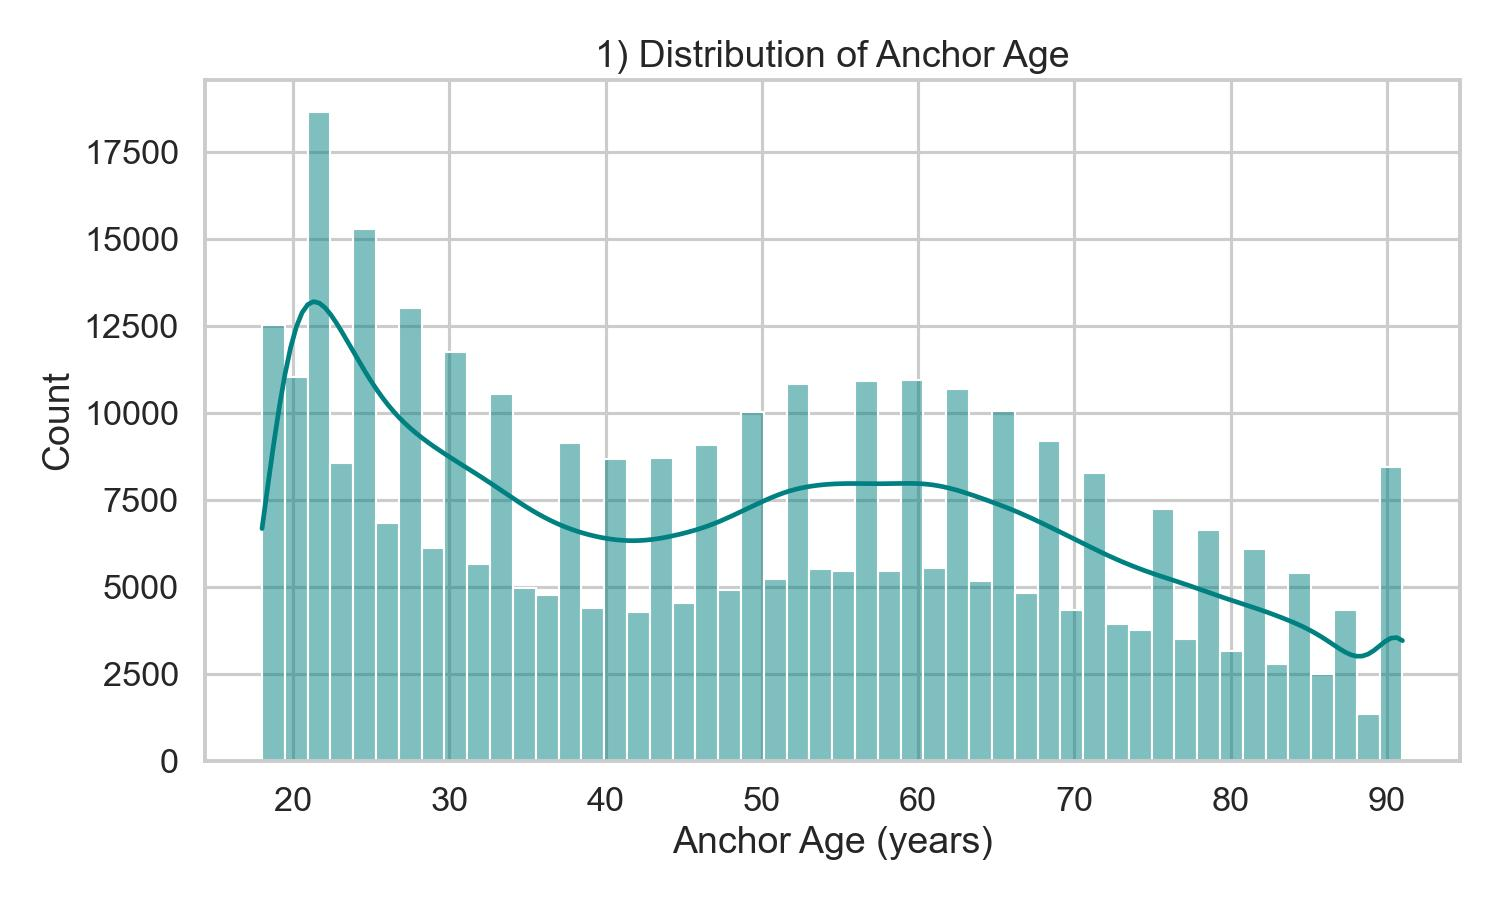
\includegraphics[width=0.5\textwidth]{mimic_plots/plot1.jpg}
    \caption{A histogram revealing a right-skewed distribution of anchor ages, with many individuals in their 20s and 30s.}
    \label{fig:plot1}
\end{figure}

\noindent
Figure~\ref{fig:plot1} shows how anchor ages are concentrated in younger to middle-aged adults, with a tail that extends to the maximum capped age of 91. There is a gradual decrease in frequency after middle age, but a mild uptick near 90--91, reflecting censoring of ages above 89.

\newpage

\subsection*{Plot 2: Boxplot of Anchor Age by Admission Type}
\begin{figure}[H]
    \centering
    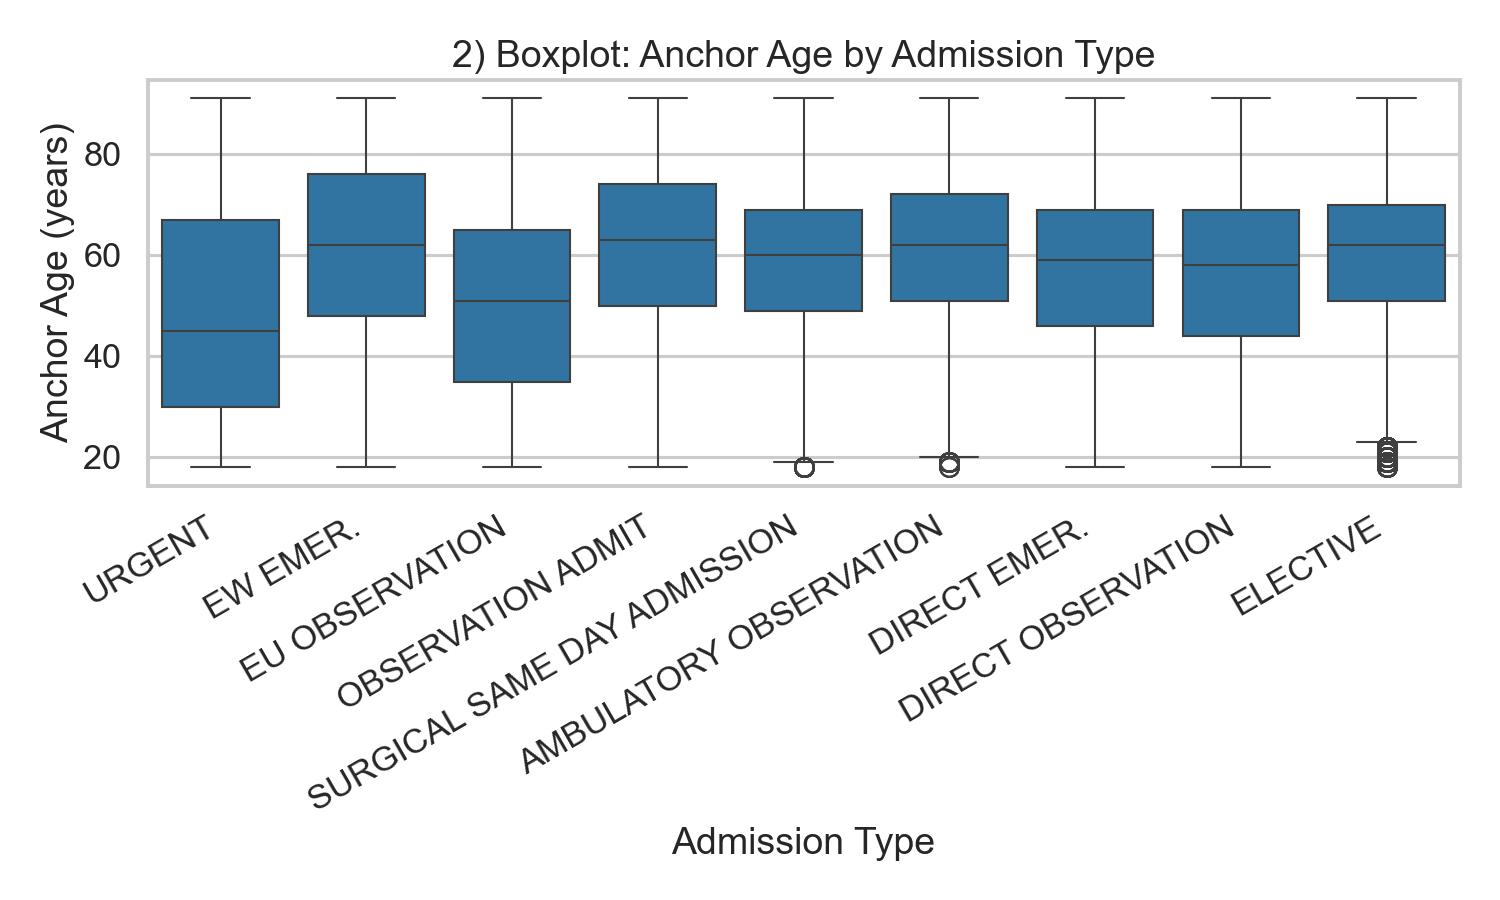
\includegraphics[width=0.5\textwidth]{mimic_plots/plot2.jpg}
    \caption{A boxplot illustrating how anchor age varies across different admission types.}
    \label{fig:plot2}
\end{figure}

\noindent
Figure~\ref{fig:plot2} offers insight into differences in age distributions for various hospital admission pathways (e.g., emergency admissions vs. elective surgeries). Some admission types span a broader age range, while others are more narrowly distributed, reflecting the patient populations associated with particular clinical services.

\newpage

\subsection*{Plot 3: Admissions by Anchor Year Group}
\begin{figure}[H]
    \centering
    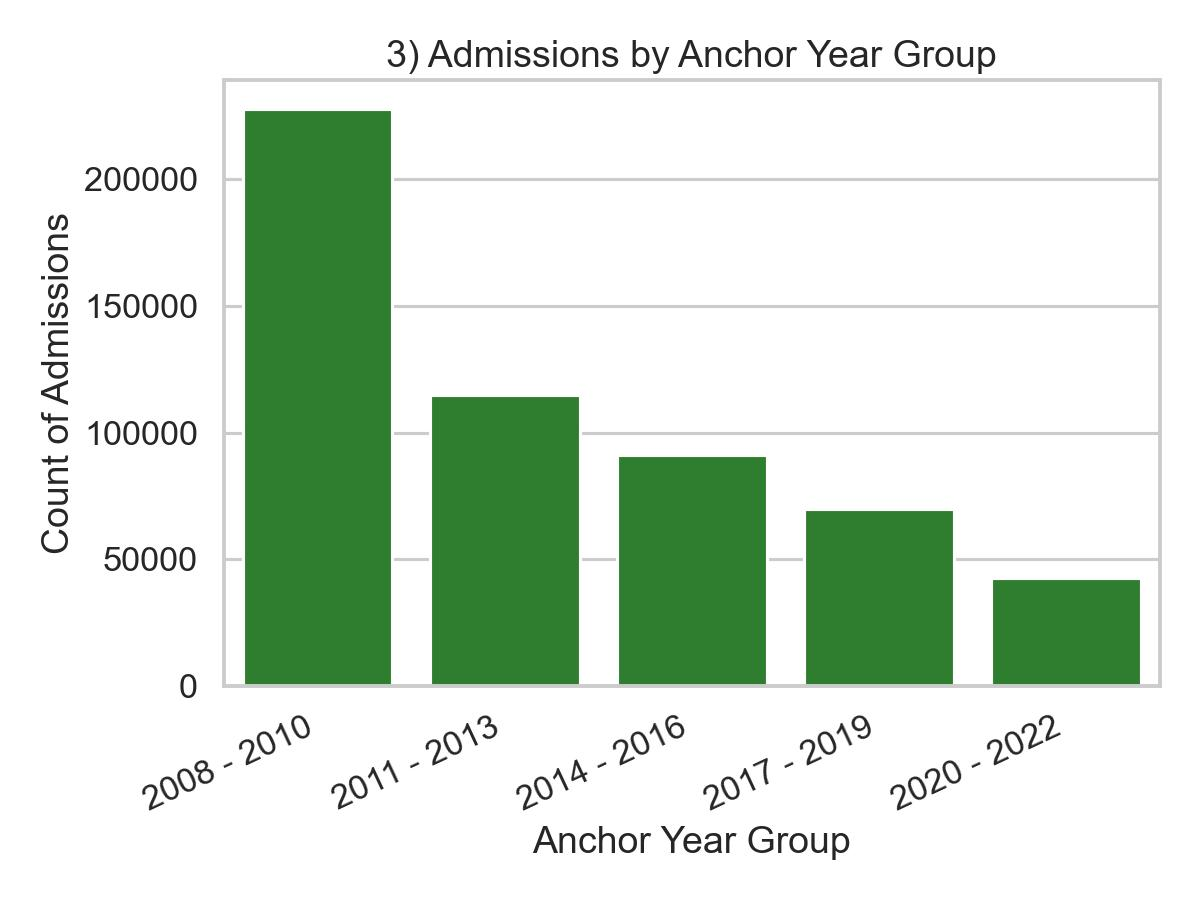
\includegraphics[width=0.5\textwidth]{mimic_plots/plot3.jpg}
    \caption{A bar chart showing the number of admissions categorized by approximate calendar year groups.}
    \label{fig:plot3}
\end{figure}

\noindent
Figure~\ref{fig:plot3} demonstrates a higher number of admissions in the earlier year intervals (2008--2010, 2011--2013) relative to later groups, likely reflecting the data collection periods and any changes in hospital practices over time.

\newpage

\subsection*{Plot 4: Top 15 ICD-10 Codes by Frequency}
\begin{figure}[H]
    \centering
    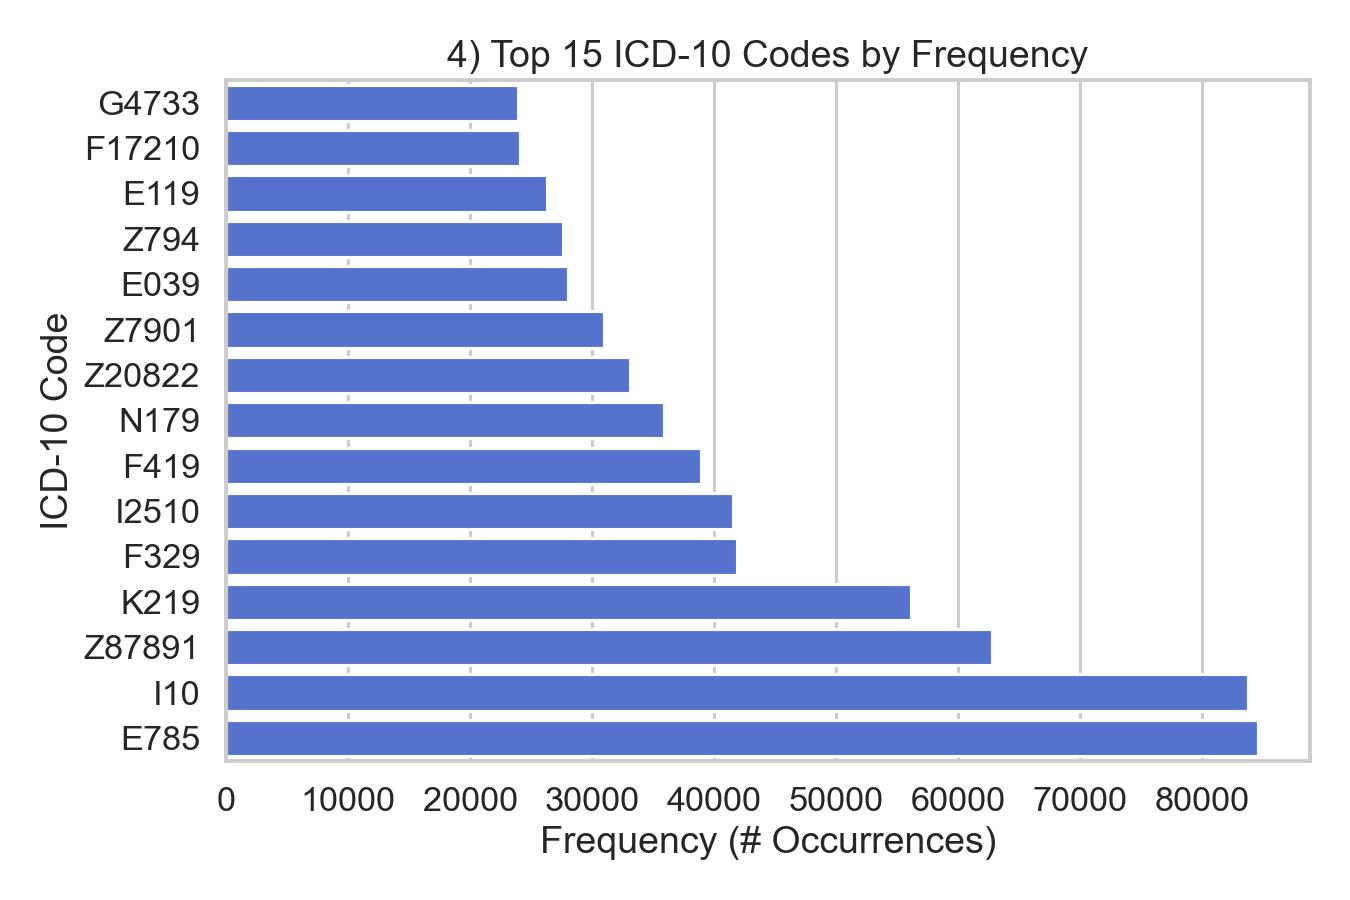
\includegraphics[width=0.5\textwidth]{mimic_plots/plot4.jpg}
    \caption{A horizontal bar chart showing the most common ICD-10 codes among admissions.}
    \label{fig:plot4}
\end{figure}

\noindent
In Figure~\ref{fig:plot4}, chronic conditions such as hyperlipidemia (\texttt{E785}) and hypertension (\texttt{I10}) are clearly visible at the top of the frequency distribution, demonstrating the widespread prevalence of these diagnoses.

\newpage

\subsection*{Plot 5: Co-Occurrence Matrix of Top 15 ICD-10 Codes}
\begin{figure}[H]
    \centering
    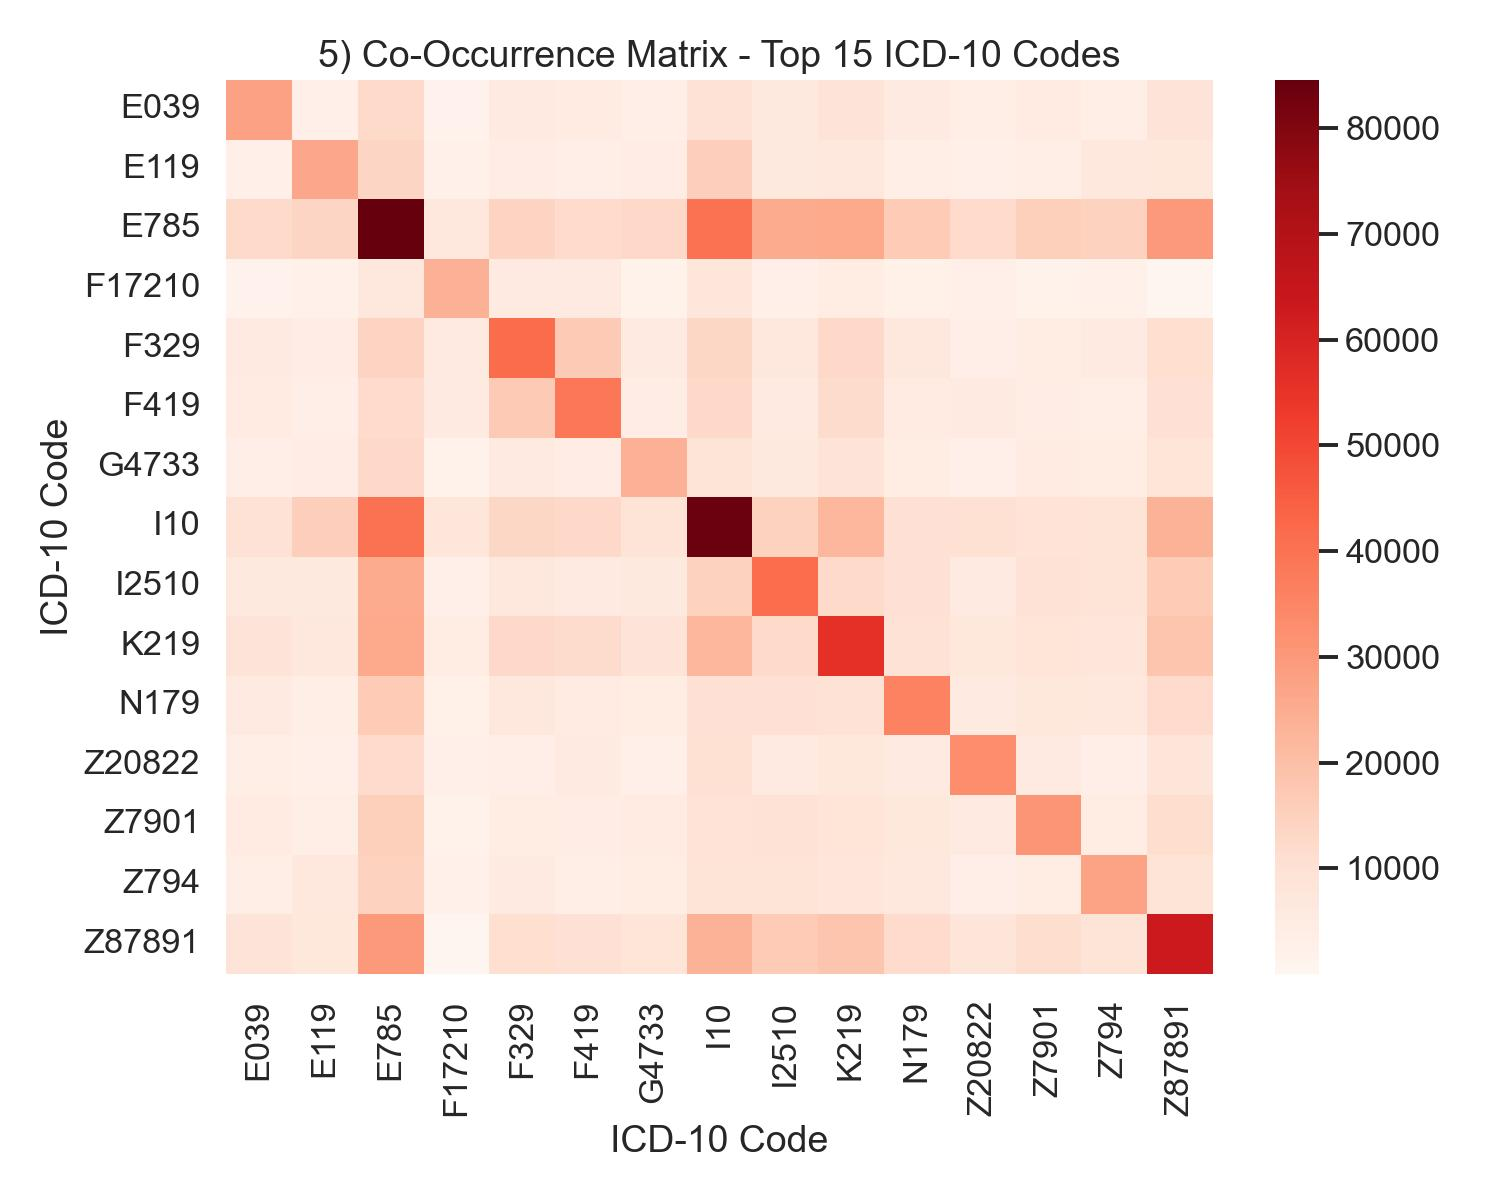
\includegraphics[width=0.5\textwidth]{mimic_plots/plot5.jpg}
    \caption{A heatmap illustrating how frequently pairs of the top 15 ICD-10 codes co-occur within the same admission.}
    \label{fig:plot5}
\end{figure}

\noindent
Figure~\ref{fig:plot5} reveals strong comorbidity patterns among high-frequency diagnoses. For instance, codes associated with hyperlipidemia often co-occur alongside hypertension, reflecting typical chronic disease clusters.

\newpage

\subsection*{Plot 6: Discharge Note Length vs. Number of ICD-10 Codes}
\begin{figure}[H]
    \centering
    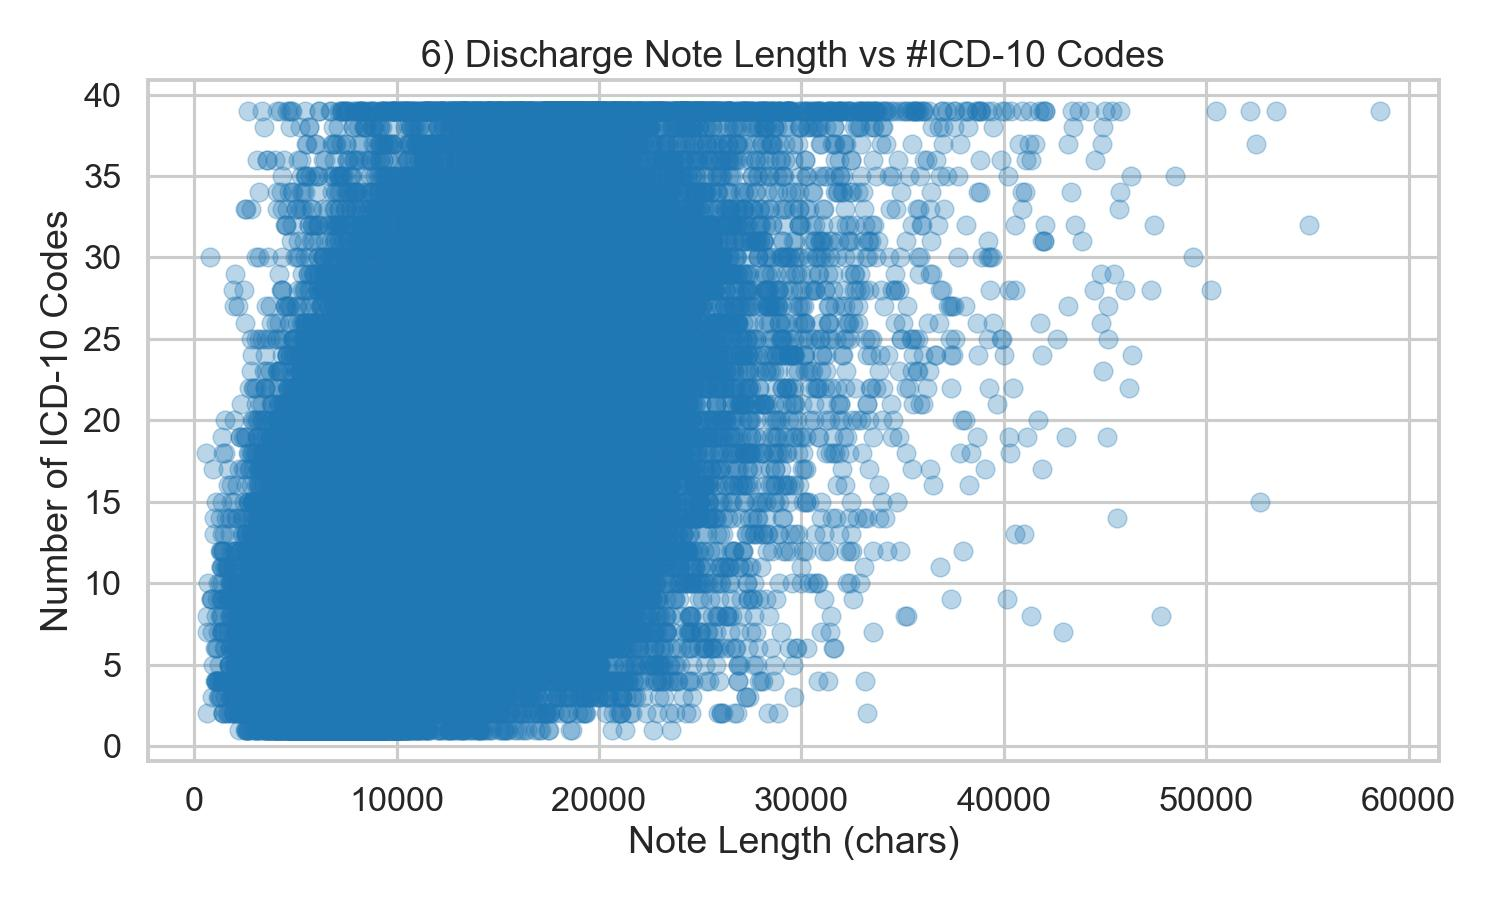
\includegraphics[width=0.5\textwidth]{mimic_plots/plot6.jpg}
    \caption{A scatter plot highlighting the relationship between note length (in characters) and the number of ICD-10 codes.}
    \label{fig:plot6}
\end{figure}

\noindent
Figure~\ref{fig:plot6} demonstrates a positive correlation: admissions with more diagnoses often generate longer discharge summaries. However, many cases are concentrated below 20,000 characters, indicating that moderately sized notes can still have multiple codes.

\newpage

\subsection*{Plot 7: Violin Plot of Code Counts by Anchor Year Group}
\begin{figure}[H]
    \centering
    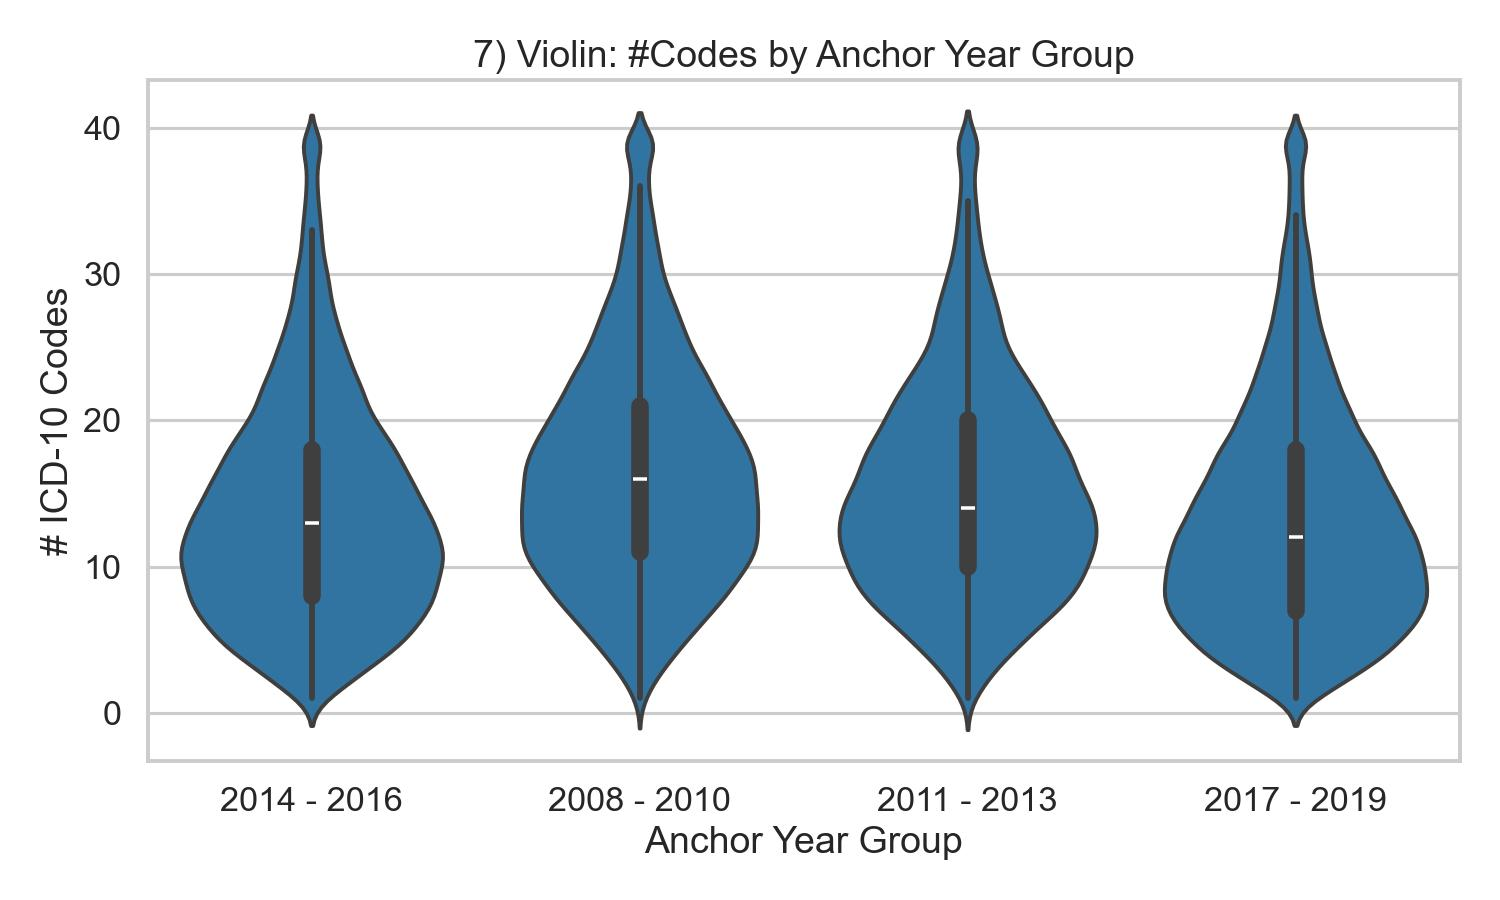
\includegraphics[width=0.5\textwidth]{mimic_plots/plot7.jpg}
    \caption{A violin plot representing how the distribution of total ICD-10 codes per admission varies across anchor year groups.}
    \label{fig:plot7}
\end{figure}

\noindent
Figure~\ref{fig:plot7} visualizes the spread of ICD-10 code counts for each time interval. Wide tails indicate that certain admissions receive a very large number of codes, reflecting complex clinical circumstances.

\newpage

\subsection*{Plot 8: Mean Discharge Note Length by Anchor Year Group}
\begin{figure}[H]
    \centering
    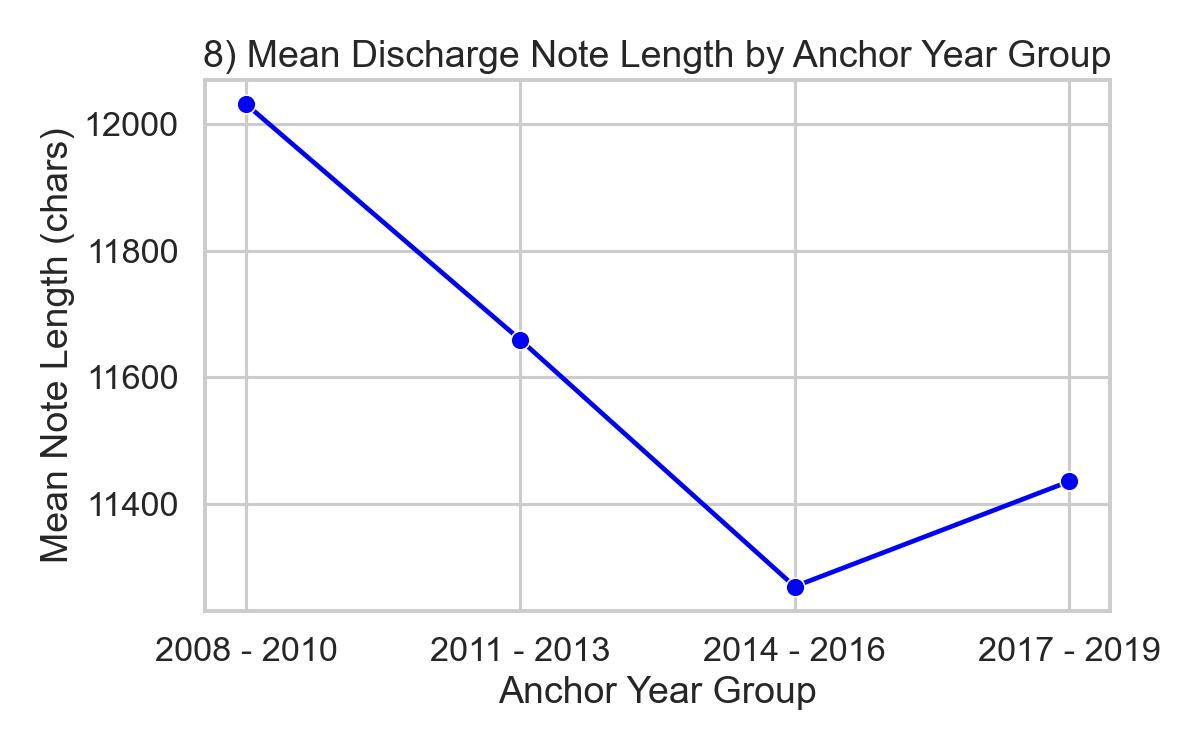
\includegraphics[width=0.5\textwidth]{mimic_plots/plot8.jpg}
    \caption{A line plot tracking average discharge summary lengths over five anchor year group intervals.}
    \label{fig:plot8}
\end{figure}

\noindent
Figure~\ref{fig:plot8} suggests that longer average notes were generated during the earlier collection periods (2008--2010), followed by a dip in 2014--2016 and a partial rebound in later intervals. Evolving clinical documentation practices may contribute to these shifts.

\newpage

\subsection*{Plot 9: Top 10 Admission Types by Volume}
\begin{figure}[H]
    \centering
    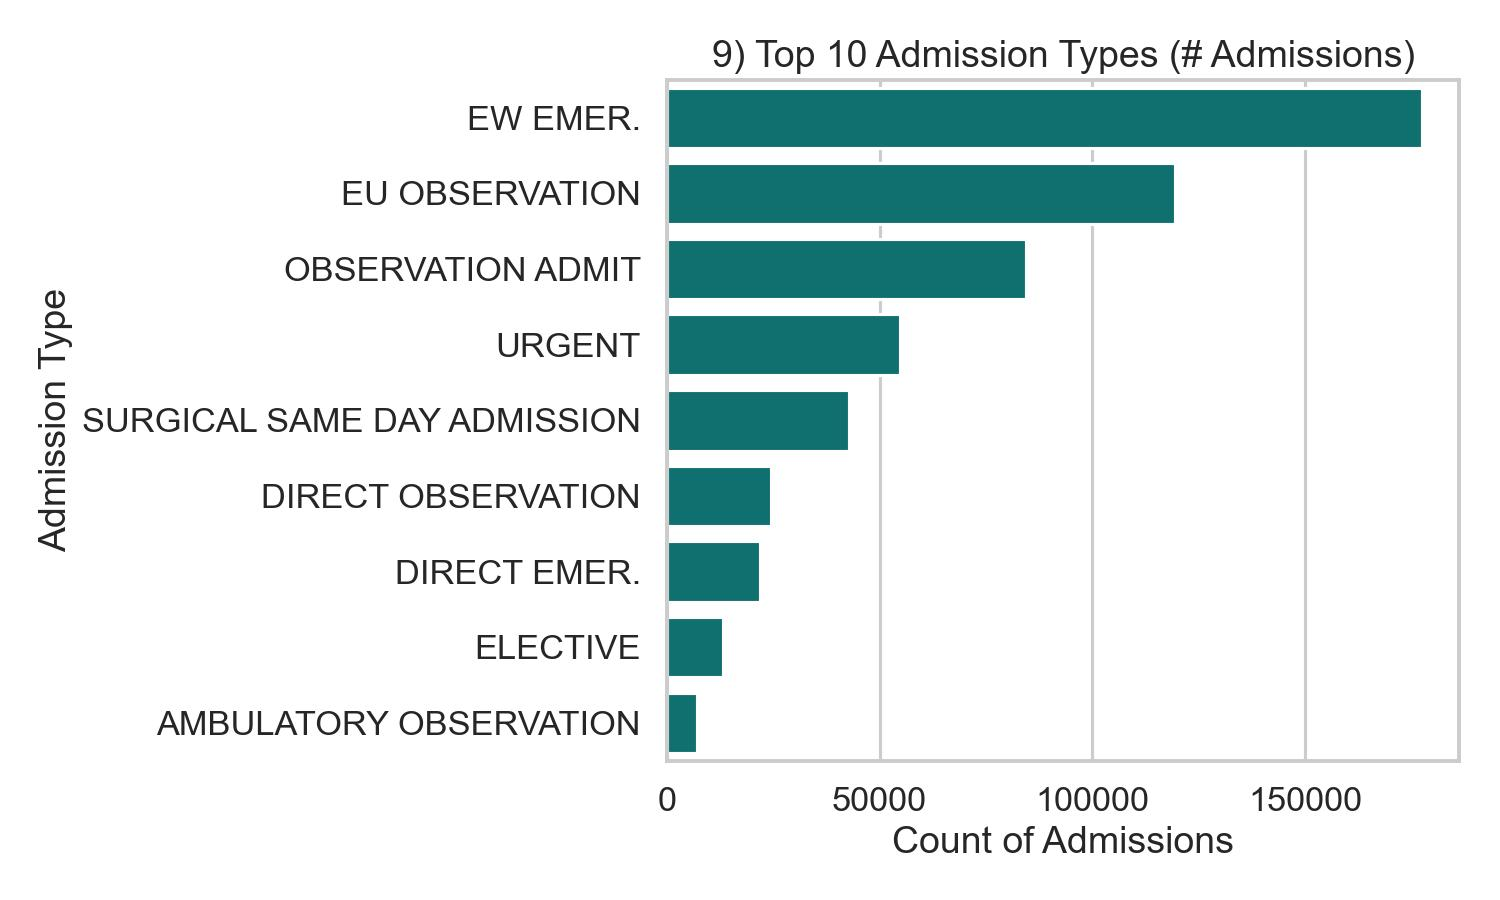
\includegraphics[width=0.5\textwidth]{mimic_plots/plot9.jpg}
    \caption{A horizontal bar chart showing the top ten admission types (e.g., emergency, elective, urgent).}
    \label{fig:plot9}
\end{figure}

\noindent
Figure~\ref{fig:plot9} highlights the prominence of emergency or unplanned admissions. Emergency admissions dominate, but there are also notable volumes in scheduled categories such as elective surgeries.

\newpage

\subsection*{Plot 10: ICD-10 Code Frequency by Anchor Year Group (Top 15 Codes)}
\begin{figure}[H]
    \centering
    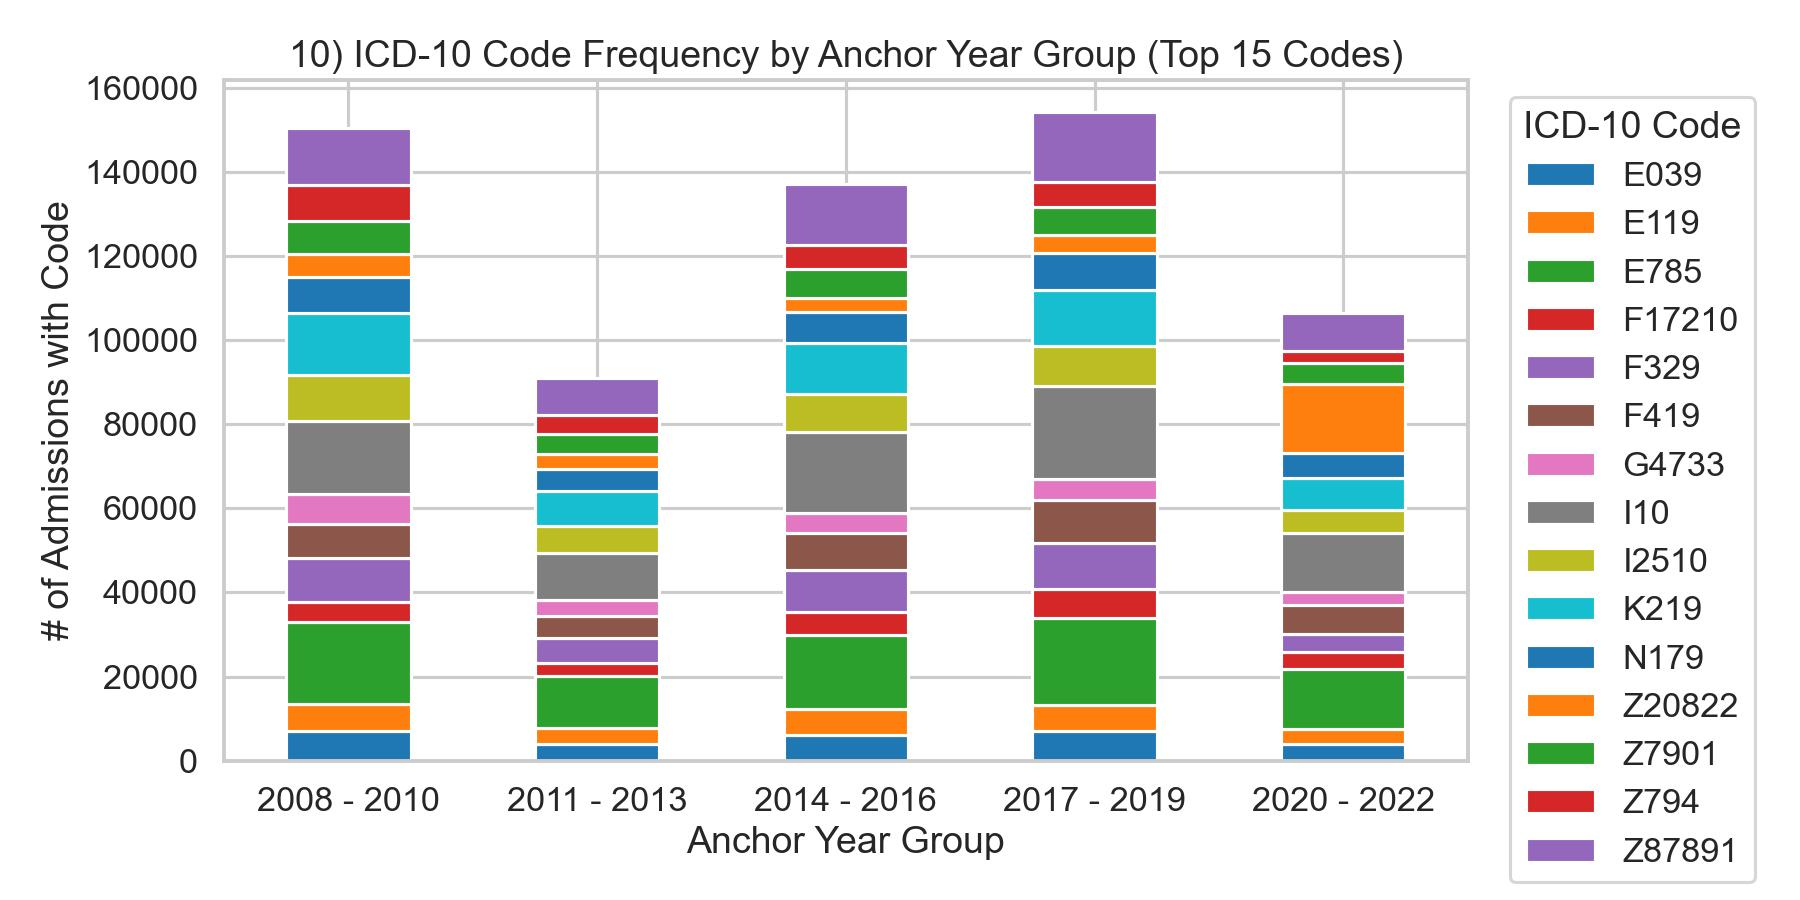
\includegraphics[width=0.5\textwidth]{mimic_plots/plot10.jpg}
    \caption{A stacked bar chart displaying the occurrence of each top-15 ICD-10 code within different anchor year groups.}
    \label{fig:plot10}
\end{figure}

\noindent
Figure~\ref{fig:plot10} shows that certain diagnoses remain consistently frequent across all anchor year intervals, again reflecting the prevalence of long-standing chronic conditions such as metabolic disorders and cardiovascular disease.

\section{Key Insights}
\noindent
From these queries and visualizations, several points emerge:
\begin{itemize}
    \item \textbf{Large-Scale Data:} There are more than 364k unique patients and over 546k admissions, providing robust coverage of a hospital population.
    \item \textbf{Multiple Diagnoses:} The average admission carries more than 13 ICD-10 codes, confirming a multi-label setting.
    \item \textbf{Long-Tail Challenge:} Over 9,217 ICD-10 codes appear fewer than five times, highlighting difficulties with rare or specialized diagnoses.
    \item \textbf{Varied Note Lengths:} Discharge summaries range from brief texts to lengthy narratives with thousands of words.
\end{itemize}

\section{Final Data Preparation}
\label{sec:final_data_preparation}
\noindent
For the goal of building a text-to-ICD coding model (akin to AWS Comprehend Medical or other automated medical coding applications), a consolidated table was created that merges each admission’s discharge note with the set of associated ICD-10 codes. The approach takes each row in the \texttt{discharge} table, then joins it with the corresponding entries in \texttt{diagnoses\_icd} for that \texttt{hadm\_id}. 

\vspace{5pt}
\noindent
The query used to accomplish this is shown in Figure~\ref{fig:sql12_merge_notes_codes} in the Appendix. Each row in the resulting table contains:
\begin{itemize}
    \item \textbf{notes}: The original discharge summary (raw text).
    \item \textbf{icd\_codes}: A comma-separated list of all ICD-10 codes assigned to that admission.
\end{itemize}

\vspace{5pt}
\noindent
This design directly supports multi-label classification, as the full narrative of the discharge summary is provided (with no additional demographic or structural metadata) alongside all billed ICD-10 codes. Such a format simulates real-world scenarios in which only free-text documentation is available for downstream coding or NLP tasks.
